% prelab2
\documentclass{IEEEtran}
\usepackage{booktabs}
\usepackage{graphicx}
\usepackage{fancyhdr}
\usepackage{framed}
\usepackage{siunitx}
\pagestyle{fancy}
\lhead{}
\chead{}
\rhead{}
\lfoot{}
\cfoot{}
\rfoot{\thepage}
\title{Prelab 2 Amplifiers}
\author{Group 8: Muhan Li \and Man Sun \and Mingxiao An \\ EE233 Circuit Theory}
\IEEEaftertitletext{\centering \vspace{-10pt} \fontsize{11}{11}\textsc{Department of Electrical Engineering, University of Washington, Seattle, WA, 98195} \vspace{10pt}}

\begin{document}
	
	\maketitle
	
	\section{\textbf{Prelab\#1}}
	The typical values of parameters of \textit{LM148} are shown in table[\ref{tab:pl1}], figure[1], and figure[2].
	
	\begin{table}[!htbp]
		\centering
		\caption{The typical values of parameters}
		\begin{tabular}{lcl}
			\toprule
			Parameter & value & \\
			\midrule
			Power supplies & $\pm22\si{V}$ & \\
			Input resistance & $2.5\si{M\Omega}$ & \\
			Slew rate & $0.5\si{V/\mu s}$ & \\
			\bottomrule
		\end{tabular}
		\label{tab:pl1}
	\end{table}
	
	\begin{figure}[!htbp]
		\centering
		\label{fig:101}
		\begin{framed}
			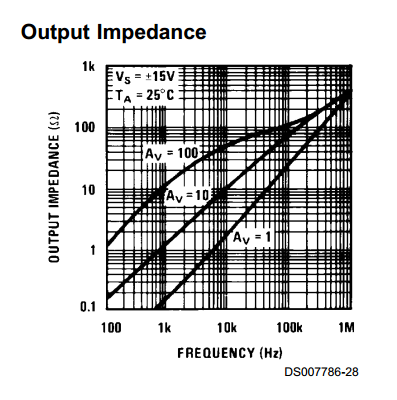
\includegraphics[width=\linewidth]{images/1_1.PNG}
			\caption{Output impedance}
		\end{framed}
	\end{figure}
	
	\begin{figure}[!htbp]
		\centering
		\label{fig:102}
		\begin{framed}
			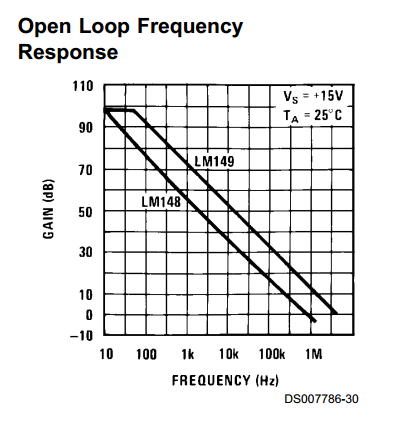
\includegraphics[width=\linewidth]{images/1_2.PNG}
			\caption{Open-loop voltage gain}
		\end{framed}
	\end{figure}
	
	\section{\textbf{Prelab\#2}}
	\begin{equation}
		\mathrm{gain} = \frac{V_{\mathrm{out}}}{V_{\mathrm{in}}} = 1
	\end{equation}
	
	\section{\textbf{Prelab\#3}}
	\subsection{Calculate the time}
	\begin{equation}
		t = \frac{\Delta V}{\mathrm{SlewRate}}
		= \frac{10\si{V}-(-10\si{V})}{0.5\si{V/\mu s}} = 40\si{\mu s}
	\end{equation}
	\subsection{Result comparison}
	The time we read from the datasheet is the gap between the two marked lines on figure[3]. It is $40\si{ms}$, so we have an error of $0.0\%$. Temperatures, or input resistance, can contribute to error between the theoretical value and actual value.
	
	\begin{figure}[!htbp]
		\centering
		\begin{framed}
			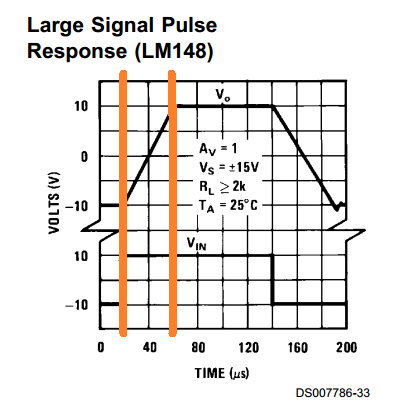
\includegraphics[width=\linewidth]{images/3_1.PNG}
			\caption{Large signal pulse response}
		\end{framed}
	\end{figure}
	
	\section{\textbf{Prelab\#4}}
	\subsection{The expression for the slope of the output voltage}
	\begin{eqnarray}
		\bigg|\frac{\mathrm{d}V_{\mathrm{out}}}{\mathrm{d}t}\bigg| & = & \bigg|\frac{\mathrm{d}V_{\mathrm{in}}}{\mathrm{d}t}\bigg| = \bigg|\frac{\mathrm{d}A\cos(\omega t + \phi)}{\mathrm{d}t}\bigg| \\
		& = & A\omega|\sin(\omega t+\phi)| \\
		& = & 2\pi Af|\sin(2\pi ft+\phi)|
	\end{eqnarray}
	\subsection{The maximum slope of output voltage}
	\begin{equation}
		\bigg|\frac{\mathrm{d}V_{\mathrm{out}}}{\mathrm{d}t}\bigg| = 2\pi Af|\sin(2\pi ft+\phi)| \le 2\pi Af
	\end{equation}
	\subsection{The maximum frequency}
	\begin{eqnarray}
		2\pi Af & \le & SlewRate = 0.5\si{V/\mu s} \\
		f & \le & \frac{0.5\si{V/\mu s}}{2\pi A}
	\end{eqnarray}
	\subsection{The maximum amplitude}
	\begin{eqnarray}
		2\pi Af & \le & SlewRate = 0.5\si{V/\mu s} \\
		A & \le & \frac{0.5\si{V/\mu s}}{2\pi f}
	\end{eqnarray}
	
	\section{\textbf{Prelab\#5}}
	\begin{eqnarray}
		A_{f=100\si{Hz}} & \le & 795.8\si{V} \\
		A_{f=5\si{KHz}} & \le & 15.9\si{V}
	\end{eqnarray}
		
	Since the voltage of audio signals is typically under 2V, which is much lower than $15.9\si{V}$. Thus, we should not be concern about it.
	
	\section{\textbf{Prelab\#6}}
	\subsection{The equation for the circuit gain}
	\begin{eqnarray}
		V_{\mathrm{out}} & = & A_v(V_+-V_-) \\
		V_- & = & V_{\mathrm{in}} \\
		V_+ & = & V_{\mathrm{out}} \\
		\mathrm{gain} = \frac{V_{\mathrm{out}}}{V_{\mathrm{in}}} & = & \frac{V_-}{V_+} = \frac{A_v}{1 + A_v}
	\end{eqnarray}
	\subsection{The value of $A_v$ when $V_{\mathrm{out}}/V_{\mathrm{in}}$ equal 0.5}
	\begin{equation}
		A_v = \frac{1}{1-\frac{V_{\mathrm{out}}}{V_{\mathrm{in}}}} - 1 = 1
	\end{equation}
	\subsection{The value of frequency when $V_{\mathrm{out}}/V_{\mathrm{in}}$ equal 0.5}
	\begin{equation}
		A(\si{dB}) = 20\log_{10}{A}
	\end{equation}
	\phantom{ } When $A_v=1$, $A$ is about $0\si{dB}$. According to the plot on the spec, $f_{A=0}$ is $7.6\times10^5\si{Hz}$.
	\subsection{The range of gain for the audio signal}
	We can find that $A_v$ is monotonic decreasing to frequency. Thus, with frequency in the range of $100\si{Hz}\sim5000\si{Hz}$, $A_v$ is range from $77\si{dB}$($7079$) down to $43.38\si{dB}$($147.5$). Then, we figure out the range of gain as:
	\begin{equation}
		\frac{V_{\mathrm{out}}}{V_{\mathrm{in}}} \in [0.99327, 0.99986]
	\end{equation}
	The difference is so small that it can be ignored. Also, the gain is very close to 1, so we can reasonably regard the amplifier as ideal.
	
	\section{\textbf{Prelab\#7}}
	\subsection{The equation for $V_{\mathrm{out}}$ in the frequency domain}
	Consider KCL at the negative port of the amplifier:
	\begin{equation}
		\frac{0-V_1}{R_1} + \frac{0-V_2}{R_2} + \frac{0-V_3}{R_3} + \frac{0-V_{\mathrm{out}}}{R_f} + \frac{0-V_{\mathrm{out}}}{\frac{1}{\mathbf{j}\omega L}} = 0
	\end{equation}
	Finally, we got the equation for $V_{\mathrm{out}}$ as:
	\begin{equation}
		V_{\mathrm{out}} = \bigg(\frac{V_1}{R_1} + \frac{V_2}{R_2} + \frac{V_3}{R_3}\bigg) \frac{-R_f}{\mathbf{j}2\pi fCR_f+1}
	\end{equation}
	\subsection{The expression for the magnitude of the output signal}
	To compute the magnitude of $V_{\mathrm{out}}$, we have following procedures:\\
	\begin{eqnarray}
		|V_{\mathrm{out}}| & = & \bigg|\frac{V_1} {R_1}+\frac {V_2}{R_2}+\frac{V_3}{R_3}\bigg|
		\frac{|-R_f|}{|\mathbf{j}2\pi fCR_f+1|}\\
		& = & \bigg(\frac{|V_1|}{R_1} + \frac{|V_2|}{R_2} + \frac{|V_3|}{R_3}\bigg) \frac{R_f}{\sqrt{1+
		4\pi^2C^2R_f^2f^2}}
	\end{eqnarray}
	\section{\textbf{Prelab\#8}}
	\subsection{Find the expression for $V_{\mathrm{out}}$ if all the inputs are DC.}
	When all the inputs are DC, we can easily derive to the conclusion that\\
	\begin{equation}
		|V_i| = V_i \mathrm{\ \ \ for\ } i = 1,2,3
		f = 0
	\end{equation}
	Hence, we have the result that\\
	\begin{equation}
		|V_{\mathrm{out}}| = \bigg(\frac{V_1}{R_1} + \frac{V_2}{R_2} + \frac{V_3}{R_3}\bigg)R_f
	\end{equation}
	\subsection{Find the frequencies for 70\% the DC value}
	We eliminate the $\bigg(\frac{V_1}{R_1} + \frac{V_2}{R_2} + \frac{V_3}{R_3}\bigg)$ part from both sides to save some space:\\
	\begin{eqnarray}
		 \frac{R_f}{\sqrt{1 + 4\pi^2C^2R_f^2f^2}}& = & 0.7 R_f\\
		\sqrt{1 + 4\pi^2C^2R_f^2f^2} & = & \frac{10}{7}\\
		4\pi^2C^2R_f^2f^2 & = & \frac{51}{49}\\
		(f>0)\ f & = & \frac{\sqrt{51}}{14\pi CR_f}
	\end{eqnarray}
	\subsection{Find the frequencies for 50\%,30\%,10\% the DC value}
	Let $k$ be the ratio of output voltage and input DC value, we can derive a formula from the computation in Prelab \#8b that:\\
	\begin{equation}
		f = \frac{\sqrt{k^{-1}-1}}{2\pi CR_f}
	\end{equation}
	So by simply changing the value of $k$, we can easily compute the frequencies:\\
	\begin{eqnarray}
		f_{50\%} = \frac{\sqrt{0.5^{-1}-1}}{2\pi CR_f} = \frac{1}{2\pi CR_f}\\
		f_{30\%} = \frac{\sqrt{0.3^{-1}-1}}{2\pi CR_f} = \frac{\sqrt{\frac{7}{3}}}{2\pi CR_f}\\
		f_{10\%} = \frac{\sqrt{0.1^{-1}-1}}{2\pi CR_f} = \frac{3}{2\pi CR_f}
	\end{eqnarray} 
	\section{\textbf{Prelab\#9}}
	\subsection{Find $V_1$, $V_2$, and $V_3$ in the phasor domain.}
	$\mathbf{@} f = 1\mathrm{kHz}$
	\begin{eqnarray}
		V_1 & = & 1\angle 0^{\circ}\\
		V_2 & = & 0.1\angle -30^{\circ}\\
		V_3 & = & 0.1\angle 30^{\circ}
	\end{eqnarray}
	\subsection{Plot the magnitude and phase of the output signal in the range from 10Hz to 1MHz.}
	See our result from figure[4]\\
	\begin{figure}
		\centering
		\label{fig:901}
		\begin{framed}
			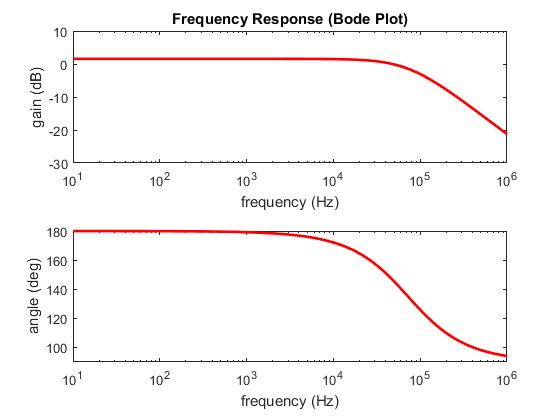
\includegraphics[width=\linewidth]{images/9_1.PNG}
			\caption{magnitude and phase of the output signal}
		\end{framed}
	\end{figure}
	\subsection{Analysis when the capacitor is removed}
	If the capacitor is removed, the magnitude of output voltage no longer depend on frequency. Because without 
	the capacitor, the magnitude of the output voltage will become $\bigg(\frac{V_1}{R_1} + \frac{V_2}{R_2} + \frac{V_3}{R_3}\bigg)R_f$, where frequency cannot affect it. The capacitor brings reactive power into the circuit and changes the magnitude of the output voltage in the phasor domain.
	\section{\textbf{Prelab\#10}}
	We followed the tutorial and simulate our circuit. The simulate result is shown in graph[5].
	\begin{figure}[!htbp]
		\centering
		\label{fig:1001}
		\begin{framed}
			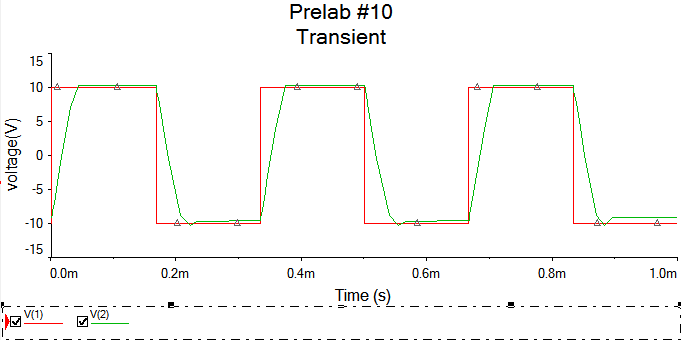
\includegraphics[width=\linewidth]{images/10_1.PNG}
			\caption{Simulate Result for Prelab \#10}
		\end{framed}
	\end{figure}
	We used cursor to measure the time interval for the output to reach the steady state after an input transition, which is shown in graph[6].
	\begin{figure}[!htbp]
		\centering
		\label{fig:1002}
		\begin{framed}
			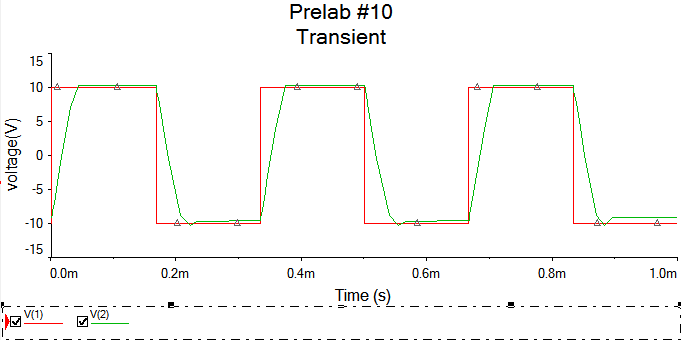
\includegraphics[width=\linewidth]{images/10_1.PNG}
			\caption{Cursor Measurement Result}
		\end{framed}
	\end{figure}
	From the graph, we can easily tell that the time interval is 44.7284$\mu$s, which is very close to our result in Prelab \#3. We can then calculate the slew rate:\\
	\begin{equation}
		\mathrm{SlewRate} = \frac{\Delta V}{\delta t} = \frac{19.3897 \si{V}}{44.7284\si{\mu s}} = 0.4335\si{V/\mu s}
	\end{equation}
	The two waveforms are very close, except that the output voltage in our simulate waveform is a little higher than the input voltage when it is in steady stage.\\
	\section{\textbf{Prelab\#11}}
	We built our circuit and simulate it according to the tutorial. Our result is shown in graph[7].\\
	\begin{figure}[!htbp]
		\centering
		\label{fig:1101}
		\begin{framed}
			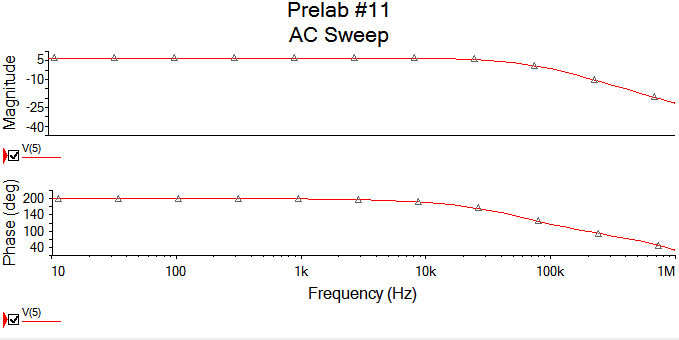
\includegraphics[width=\linewidth]{images/11_1.PNG}
			\caption{Simulate Result for Prelab \#11}
		\end{framed}
	\end{figure}
	We can see that the magnitude in two waveforms are very close, while the phase is a little bit different in high frequency. Our simulate result for phase doesn't slow down its declination greatly in high frequency while the one in Matlab does, it may be caused by the non-ideal feature of capacitor in high frequency.\\
\end{document}

